\chapter{\label{ch:instrumentation_development}Instrumentation Development}

The instrumentation exposed in the preceeding chapter was largely based on work already done by past members of my group. In this chapter, I detailed several major improvements and setup I have, partially or completely, achieved during my thesis. In this regard, I will firstly outline the measurement protocol I have implemented in the cryogenic setup to at temperatures outside the normal operating condition. Secondly, I will

\section{Temperature-dependent Protocol}

Dilution refrigerators are suited for cryogenic operations although it is possible to operate at higher temperature by working with still and mixing chamber heaters. In order to measure reliably up to room temperatuer, however, one must ensures that the temperature drift is ideally slower than the time taken to acquire experimental measurements. Since there is no well-defined experimental procedure for doing so, a workaround which leverages the Triton system was found in this thesis.

% Triton heaters are capable to control the temperature precisely from base temperature ($\sim$ 25 mK) up to 30 K. In order to stabilise the temperature above this range, one has to generate a thermal link between the sample and the environment. First the heaters (mixing chamber and still, see Ch.~\ref{ch:theory}) are switched off: this enables main heat sources to be excluded from exchanging thermal energy with the sample inside the mixing chamber. Being the mixing chamber very well thermally isolated, the temperature will start raising very slowly: to give a reference number, $\sim$24h after the heaters were switched off the temperature rose by only 2 K. The pre-cooling loop is then filled with the He3/He4 mixture, creating a thermal link between the various stages within the dilution refrigerator and the mixing chamber. This results in a faster heating rate, but slow enough to allow to take quick measurements such as $I-V_\textrm{SD}$ and $I-V_\textrm{G}$ traces.

% While these kind of measurements measure the current flowing through the device (after the voltage to current conversion that occurs inside the Delft box, see Ch.~\ref{ch:theory}), it is generally reccommended to acquire also the conductance. In absence of a lock-in apparatus, a possible workaround is to measure the current at various bias voltages and different gate voltage and differentiate numerically the current to obtain the conductance. In order to stabilise the temperature and remove the thermal link between the mixing chamber and the various refrigerator stages, the pre-cooling loop in then emptied, leaving the sample thermally isolated. The whole procedure was then automated in a python python script measurements, which algorithm is detailed in Alg.~\ref{alg:cap}.
\clearpage
\begin{algorithm}[H]
    \caption{Triton High Temperature Measurement}\label{alg:cap}
    \begin{algorithmic}[1]
        \Require Initialise Alazar, Triton and IVVI
        \Ensure Alazar, Triton, and IVVI are global
        \State Initialise Final Temperature
        \State Initialise Bias Array
        \State Initialise Target Temperatures Array
        \State Current Temperature $\gets$ Read Temperature
        \State Temperature Step $\gets$ 3
        \State Temperature Channel $\gets$ 8
        \State Precooled $\gets$ \texttt{False}
        \While{Current Temperature $<$ Final Temperature}
        \State Precooled $\gets$ \texttt{True}
        \State T $\gets$ Read Temperature
        \If{T $> 1.5$ }
        \State Temperature Channel $\gets$ 5
        \EndIf
        \For{length Bias Array}
        \State Run Gate Trace Measurement
        \EndFor
        \State T $\gets$ Read Temperature
        \If{T is in Target Temperatures Array}
        \State Precooled $\gets$ \texttt{False}
        \State Run Stability Diagram
        % \State $N \gets \frac{N}{2}$  \Comment{This is a comment}
        \EndIf
        \EndWhile
    \end{algorithmic}
\end{algorithm}

The Alazar card, Triton, and IVVI (Delft box modules) drivers are first initialised and assigned to global variables which hold their state throughout the program execution. Then several variables are initialised. The precooled variables is a routine implemented directly on top of Triton drivers which allows to set and get command directly on the instruments. While below 1 K the RuO$_2$ thermoter is used, to reliably read the temperature above this temperature one has to switch to the Cernox thermometer, hence I are setting the temperature channel variable to channel 5 within the while loop in case this conditions applies. The program then acquires gate trace and stability diagram measurements. These are functions which have been implemented and improved from scripts written by a former member of the group, Dr Nicola Dotti.

% \begin{figure}[hbtp]
%     \begin{center}
%         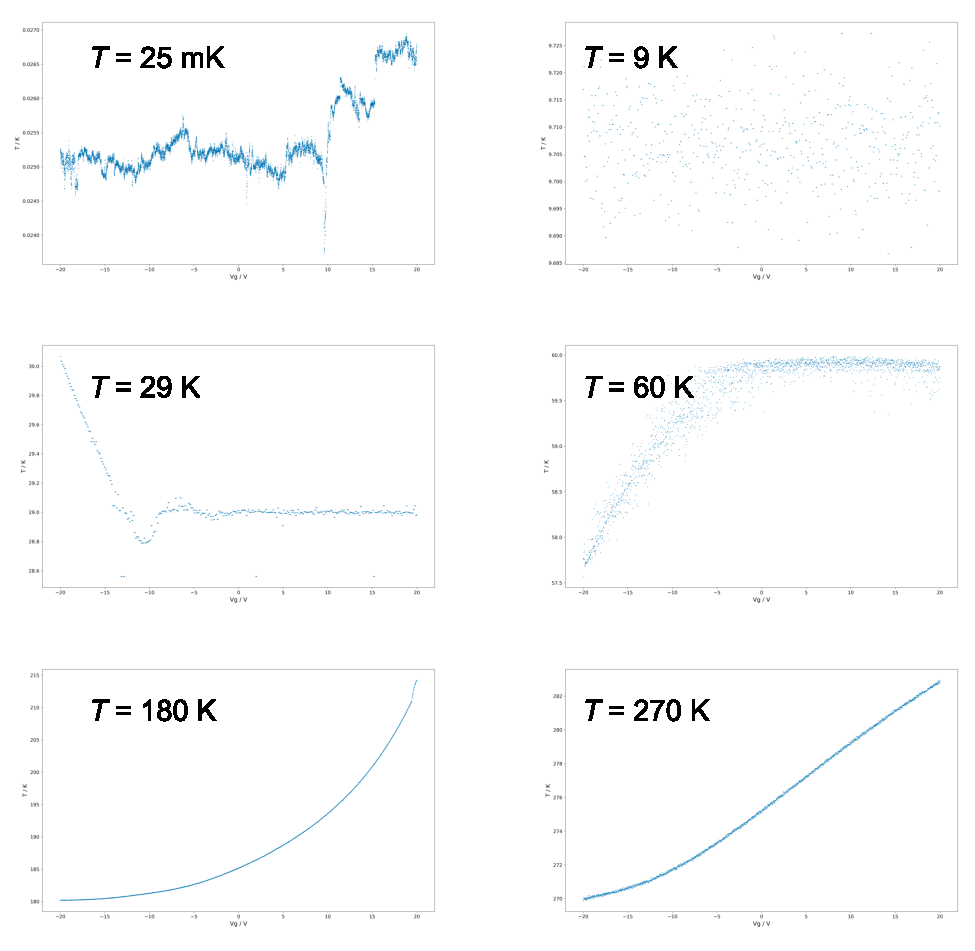
\includegraphics[width=\textwidth]{chapter_fabrication/figures/sd_progress.pdf}
%         \caption{Temperature fluctuations experienced by the cyostat over a 2-days-long stability diagram scan. From the graphs it is evident that these become more important when the temperature surpasses 30 K, which is the threshold beyond which heaters lose control over the cryostat.}
%         \label{fig:sd_progress}
%     \end{center}
% \end{figure}


\subsection{AC Measurements}

In the last part of my thesis I managed to find a workaround and integrate the lock-in amplifier to the existing setup. Previous attempt failed due to an impedance mismatch when the output from the delft-box was fed into the alazar card. While this might had beeen resolved in re-calibrating the alazar card, the signal was impossible to detect.

\begin{figure}[hbtp]
    \begin{center}
        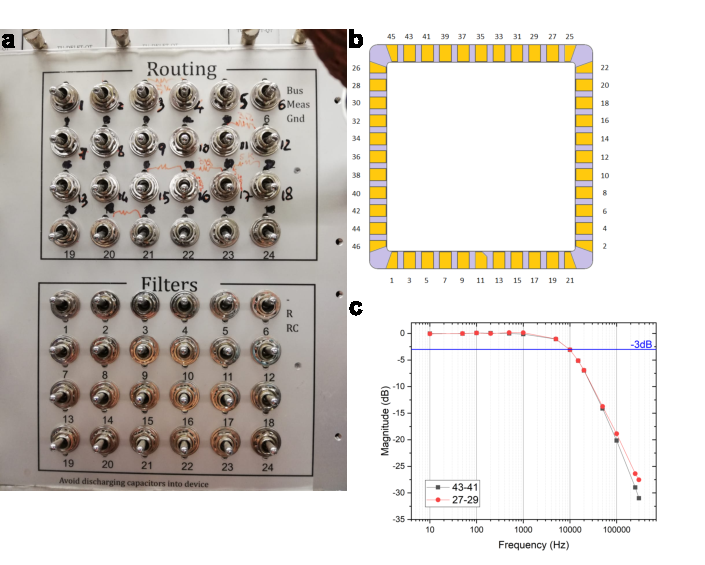
\includegraphics[width=\textwidth]{chapter_fabrication/figures/dc_lines_chipboard.pdf}
        \caption[Breakout Box Connection, Chipholder Schematic, and DC Lines Frequency Test]{\textbf{a,} Breakout box of DC connections. A second breakout box is used for connections from 26 to 48.
            \textbf{b,} Chipholder schematic with each connection numbers: pin 11 is used to orientate the chip in the correct direction.
            \textbf{c,} Frequency test. Powder (Cu) and RC filters set frequency operation limit theoretically up to \SI{10}{\kilo\hertz}. In practice we experimentally observed a statistical significance degradation of the signal already at \SI{5}{\kilo\hertz}.}
        \label{fig:dc_lines_chipboard}
    \end{center}
\end{figure}

Firstly, the module it was necessary to wire the DAC module. The standard routing do not couple the iso-amp output (S0) module with the summation module. The design is, however, convenient enough to rewrite by sampling redericting the wire as provided in the scheme. The Lock-in output was thus connected to the delft box S0, whilst fed with the signal coming out from the M0 module. The signal was then locked at the desired frequency and adjusted phase prior to be fed via usb or ethernet into the desktop computer. Experiment routines were easily written and integrated into the existing setup by simply instantiating a lock-in instance and integrating into the superclass station where instance for all the other necessary instruments are initialised and contained.

\subsubsection{Integration of Lock-in Amplifier with Delft Box}
A great deal of information about both the theory and tips of integrating a lock-in with and existing low-noise setup such as the one I have used may be found in the excellent reference \cite{lock-in_kavli}. Here I briefly report and comment salient points that I have employed to successfully integrate a standard SR-830 lcok-in with Delft Box. Same concepts were later applied for integrating two Zurich Instruments MFLI amplifier as well.

Although the measured cryogenic setup noisefloor level is a tenth of pA, the intrisic $1/f$ noise represents an instrinsic and important hurdle in any \gls{DC} experiment. As we saw in Sec.~\ref{ch2:derivation_tunneling_DOS}, the central quantity in an electron transport experiment is the tunneling density of states, which is ultimately related to the derivative of the current in a $I-V_\textrm{SD}$ experiment. Numerically retrieving the conductance may introduce noise due to the non-negligible current fluctuations between two measurement points; this picture gets even further complicated if one takes into account possible charge jumps occuring during the acquisition.

The logic behind a lock-in is as surprinsingly simple as clever. The idea is to fed an oscillating voltage $V_\textrm{osc} (f)$ into the pure \gls{DC} signal in order to produce an oscillating current $I_\textrm{tot} (f) = I_\textrm{DC} + I_\textrm{AC} (f)$ and then later to filter out the noise outside a narrow band $f \pm \tau^{-1}$ for a settable integration time $\tau$. As the reference at the top of this sections points out, lock-in conductance measurements can readily introduce errors on the scale of 10 points percent of the total signal if operated with the incorrect parameters settings, wherease \gls{DC} is not susceptible to these complex-space-caused aberrations. Therefore, it is advisable to take extra caution if accurate conductance values are required from your lock-in measurement. More loose conditions might be consider, on the contrary, if features are desired rather than accurate values.

\begin{figure}[hbtp]
    \begin{center}
        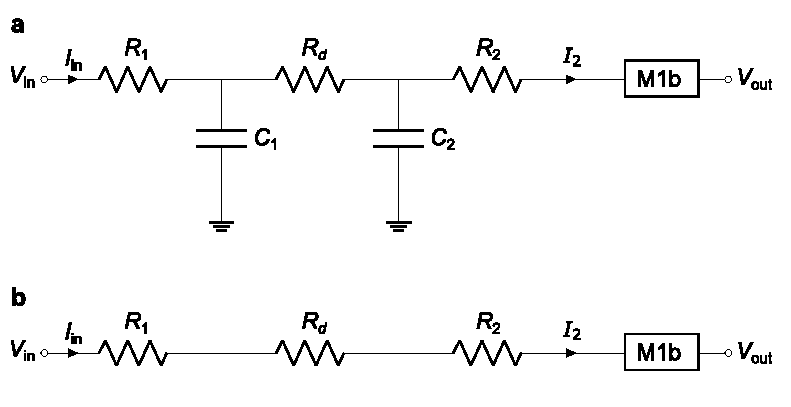
\includegraphics[width=\textwidth]{chapter_fabrication/figures/circuit_diagram_meas_fridge.pdf}
        \caption[Circuit Schematic of a Voltage-Biased Sample Thorough the Breakout Box]{
            \textbf{a,} An example of circuit diagram of a voltage-biased sample $R_d$ in series with two $RC$ filters and measured by a current-to-voltage (M1b) converter.
            \textbf{b,} Because the device resistance is finite and the operating frequency is well below the DC lines bandwidth, it is assumed that capacitors' frequency response plays no role.}
        \label{fig:exp:circuit_diagram_meas_fridge}
    \end{center}
\end{figure}


Fridge lines are filter with RC and Cu powder filter. At finite frequency $\omega =  2\pi f$, each circuit component response has to be modeled in the complex plane. As long as all the $k$ capacitors active across all the stages within the fridge do not draw any current, i.e.  $R_i \ll 1/(\omega C_k)$ where the subscript $i$ denotes the number of resistance, it is safe to exclude any parasitic components when one attempts to recover the resistance value for the device under test. The fridge bandwidth was tested

This principle might be thought as the requirements to work with oscillating voltages way below that the cut-off frequency imposed by the filters, namely:

\begin{equation}
    f \ll f_\textrm{cutoff} = \frac{1}{2\pi R_i C_k}
\end{equation}

Fig.~\ref{fig:dc_lines_chipboard}c demonstrates the cut-off frequency set by out setup to be around \SI{1}{\kilo\hertz}, even though the \SI{-3}{\decibel} point lies around one order of magnitude higher. The finite-frequency efficiency and response of the DC lines is, however, not the only factor that one has to take into account when adopting AC techiniques.

\begin{figure}[hbtp]
    \begin{center}
        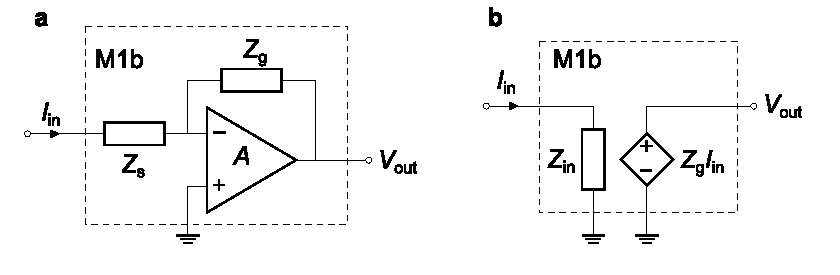
\includegraphics[width=\textwidth]{chapter_fabrication/figures/current_to_voltage_converter.pdf}
        \caption[Measuring a Noisefloor Down to \SI{5}{\unit{\pico\ampere\per\Hz\tothe{0.5}}}: Current-to-Voltage Schematic]{\textbf{a,} Current-to-Voltage simplified scehmatic. \textbf{b,} Equivalent circuit. In the M1b adopted in our setup, a manual dial allows changing $Z_g$ from \SIrange{1}{1e3}{\mega\ohm}.}
        \label{fig:exp:m1b_module}
    \end{center}
\end{figure}

Due to its narrow bandwidth of approximately \SI{200}{\kilo\hertz}, the most commonly used M1b current amplifier in the IVVI rack is especially susceptible to lock-in finite-frequency problems. Slower amplifiers require less operating current, so the objective of this amplifier's design is to minimise its back action on the sample. Nonetheless, this constrains the operating frequency to approximately \SI{30}{\kilo\hertz},\footnote[2]{The Zurich Instruments lock-in contains a built-in functionality that allows frequency sweep while monitoring the voltage noise calculated in nV/$\sqrt{\textrm{Hz}}$ for a given lock-in measurement bandwidth.}. When this condition is not met, one must consider only the features of the measurement results and not their exact values.

\section{Micro-Hall Devices}

The ability to fabricate and manipulate the properties of magnetic structures at the mesoscale has not only led to the discovery of several new physical phenomena, but also to the development of a large pool of experimental techniques for studying such structures. In this regard, the micro-probe magnetometry based on the Hall effect is of particular interest. It offers high field sensitivity even when the dimensionality shrinks down to the nanoscale, has excellent operating ranges in terms of temperature and magnetic field, and it is non-invasive.

\subsection{Technical Background}
Recalling that in order to measure the conductivity $\sigma$ of a semiconducting sample, when there are negligible gradients of carrier density, one has to take into account both the electrons concentrations $n$ and mobility $\mu_e$ and the same quantities for holes, namely:
\begin{equation}
    \sigma = \abs{e}(n\mu_e + p\mu_h) = \frac{\vec{J}_\textrm{drift}}{\vec{E}}
\end{equation}
if---while a current is flowing along the $+x$ direction---a magnetic field is applied along the $+z$ direction, the drifting holes and electrons experience an average force in the same ($-y$) direction, i.e.:
\begin{align}
    \vec{F_e} & = +\abs{e}\vec{E}\mu_e B_z \quad\text{for electrons} \\
    \vec{F_h} & = -\abs{e}\vec{E}\mu_h B_z \quad\text{for holes}
\end{align}
Note that because the electron ($\vec{v_e} = \vec{E}\mu_e$) and hole velocities are in the opposite direction, the two forces are in the same direction. When these two forces are unequal, the surfaces along the $\pm y$ of the sample become charged and a potential difference arise between them. The appearence of this voltage is the Hall effect, and was discovered in 1879 by Edwin H.\ Hall.

The transverse electric field $E_y$ builds up until the transverse force due to it becomes equal and opposite to the force due to the magnetic field. When this happens, the stationary condition $eE_y = e v_x B_z$ allows to define the Hall voltage as:
\begin{equation}
    V_\textrm{H} = wE_y = v_xB_z = \frac{j_x B_z}{ne}
\end{equation}
where $w$ in this case is the width of the semiconducting material, $j_x$ is the component along $x$ of current density and $n$ is the charge carrier density. Considering that $j = I_\textrm{SD}/wd$ where $d$ is the specimen thickness, the expression may be rewritten as:
\begin{equation}
    V_\textrm{H} = R_\textrm{H}I_\textrm{SD}B_z \quad \textrm{with}\quad R_\textrm{H} = \frac{E_y}{j_x B_z} = \frac{1}{ned}
    \label{eq:hall_coeff}
\end{equation}
From this relation it is clear that by knowing the charge carrier density one could in principle measure the   magnetic field. The minimum magnetic field detectable for a given area is called sensitivity and it is often defined as the ratio between the electrical noise and the Hall voltage.

Due to the pandemic of Covid-19 it has been impossible to find an adequate 2DEG substrate for this project. Nevertheless, I have tried to setup and detect the Hall signal from a Mn$_12$ microcrystals with a mesoscopic Hall made of Au.
The Hall probe configuration with the simplest geometry is the Hall cross. When a magnetic object is placed close to the active area of the probe, the Hall signal will be proportional to the sum of the external field $B$ and the magnetic stray field that enters the active area from the sample.

\subsection{Fabrication and Experimental Setup}
\co{Describe also here from a setup point of view which complications have raised during the setup (direct lines instead of dc lines,
    the need to use nano-D connectors and to design the a new pcb board).}

As previously observed in Sec~\ref{ch:fabrication:triton_setup}, Cu powders and low-pass filters are used to filter DC lines extensively. Therefore, it is not possible to drive sufficient current through the wire spanning the two hall bars. In addition, when the current flowing through any load is low, the power of the delft box module is significantly reduced. \footnote[2]{If the impedance of the device under test (DUT) is low, the voltage drop across is also low since the current through the resistor is large. This causes the DAC's output voltage to drop dramatically.}.

Devices used for magnetometry were fabricated by Dr Alex Gee (Fig.~\ref{fig:exp:hallbar}).

\begin{figure}[hbtp]
    \begin{center}
        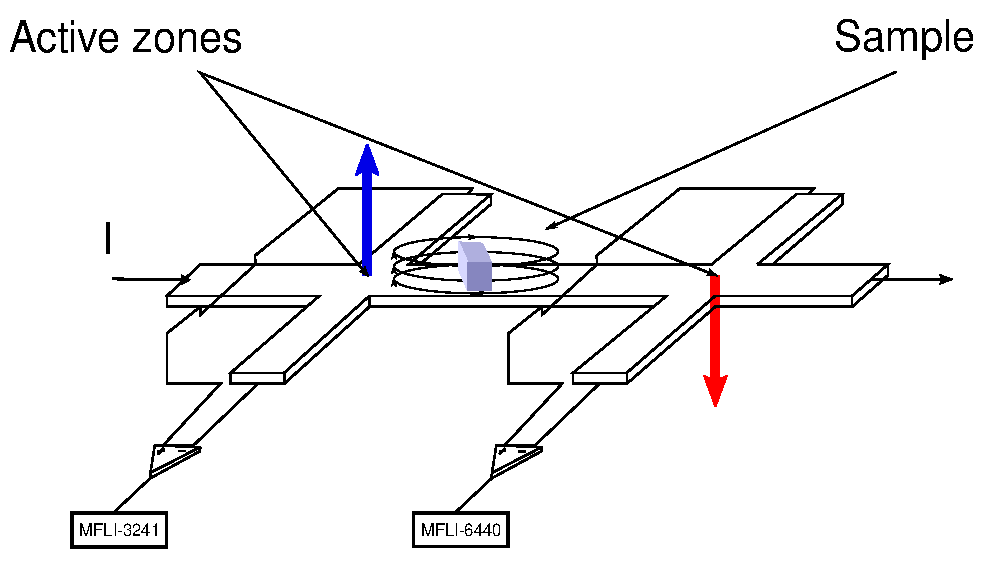
\includegraphics[width=\textwidth]{chapter_fabrication/figures/hb_sample_center.pdf}
        \caption[Micro-Hall Sensor Operating Schematic]{
            Cartoon of a micro-Hall sensor. Current flows along the central wires, while the sample sits on one of the two crosses. The sample is placed slightly offset compared to the crossposition as the magnetic field is less shielded by the gold surface. The signals are then measured in parallel by feeding first the voltage drops to two pre-amplifier and later to lock-in amplifiers.}
        \label{fig:exp:hallbar}
    \end{center}
\end{figure}

\begin{figure}[hbtp]
    \begin{center}
        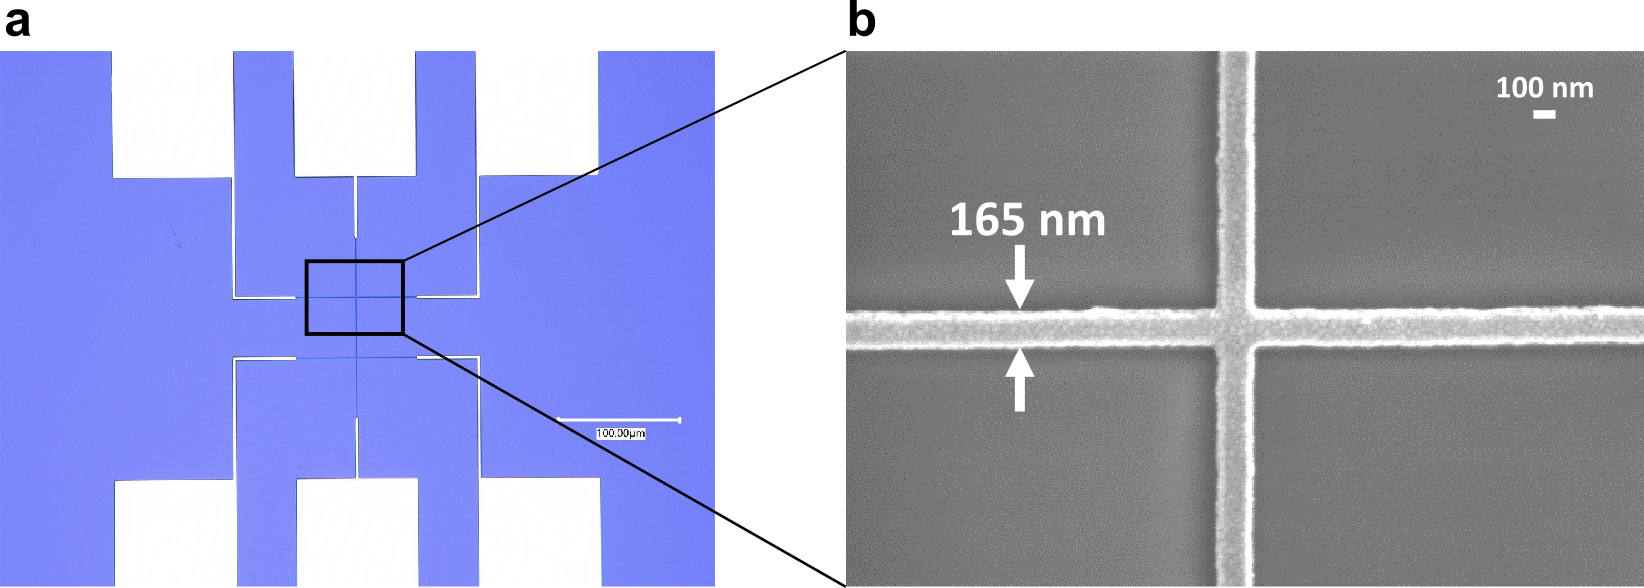
\includegraphics[width=\textwidth]{chapter_fabrication/figures/hb_design.png}
        \caption[Optical and SEM Image of a Au-Fabricated Micro-Hall Sensor]{
            \textbf{a,} Optical microscope of a double-cross Hall bar fabricated with Au. The distance betwen the two crosses for this particular devices was \SI{50}{\micro\metre}. \textbf{b,} Enlargment taken at the SEM of one of the two crosses, with the wire width displayed.}
        \label{fig:exp:hallbar_design}
    \end{center}
\end{figure}


\subsection{Test Measurements}

In order to prove the reliability of our apparatus and test its sensitivity, I have performed a few tests by measuring micro-crystals of Mn$_{12}$-acetate synthesised by Dr Dimitris Alexandropoulos. Mn$_{12}$ is a molecular magnets whose magnetic response is well known in the literature.

The coercive field of Mn$_{12}$ at cryogenic temperature is about \SI{6}{\tesla}, therefore I had to operate and temperatures higher for checking its magnetic response. In order to minimise chances the magnet would increase the temperature while was swept, I have slow sweep rates ranging from \SIrange{0.83}{1.67}{\milli\tesla\per\second}.

We used SiO$_2$ as substrate where Hall devices with different spacing between the two crosses were used, ranging from \SI{10}{\micro\metre} to \SI{50}{\micro\metre}. The deposition and the correct orientation of the crystals reavealed to be not a negligible challenge and so we choose to use crystal approximately of \SI{50}{\micro\metre}.

The transfer process was as followed. We first spread the Mn$_{12}$ crystals on top of a filter paper in order to remove big chunck of crystals. In particular, molecular monemers present a needle-shape whereas dimers comes in a bulky-ball shape form. We then deposited a few of these crystals on top of a bare silicon substrate, where we also deposited a thin film of high-vacuum grease. We then lowered one of the probe in the probe station setup as described in Sec.~\ref{fabrication:sec:probe_station} thanks to the micropositioner. Tungesten probes with a nominal diameter of \SI{10}{\micro\metre} worked best for this purpose. We then gently deposited the grease within the two crosses paying attention specifically to not to damage the electrical connections.

The probe was then cleaned, and used to pick up a Mn$_{12}$ crystal with the right lateral dimension. This was then gently lowered on top on the Hall bar device.

In order to maximise the dipolar field generated by the sample, the crystal should be perfectly oriented along the central gold pads. The difficulty of aligning the crystal in the desired direction is one of the weaknesses of our approach. Adjusting it by rotating the probe chuck is a viable alternative, but care has to be taken in not damaging the electrical connections. Another source of problem is that often the crystal break upon touching the substrate. Although monemer of Mn$_{12}$ should be relatively robust against the forces at play in this scenario, breaks might result as due to grains of crystals attached to each other.

\subsubsection{Current Measurement Test of the Hall Effect}

The first test I did was to make sure that the Hall effect was present at varying measurement bias.
From Eq.~\refeq{eq:hall_coeff} the Hall voltage $V_\textrm{H}$ is proportional to the current and the magnetic field and inversly proportional to the carrier density $n$ of the conductor.
As shown in Fig.~\ref{fig:exp:hallbar_test_current}, I have used only one lockin amplifier since only we were only intersted in the voltage built up across just one cross. The signal was then fed into a lock-in, and the digitise signal was then read directly in a standard desktop via an usb cable.

\begin{figure}[hbtp]
    \begin{center}
        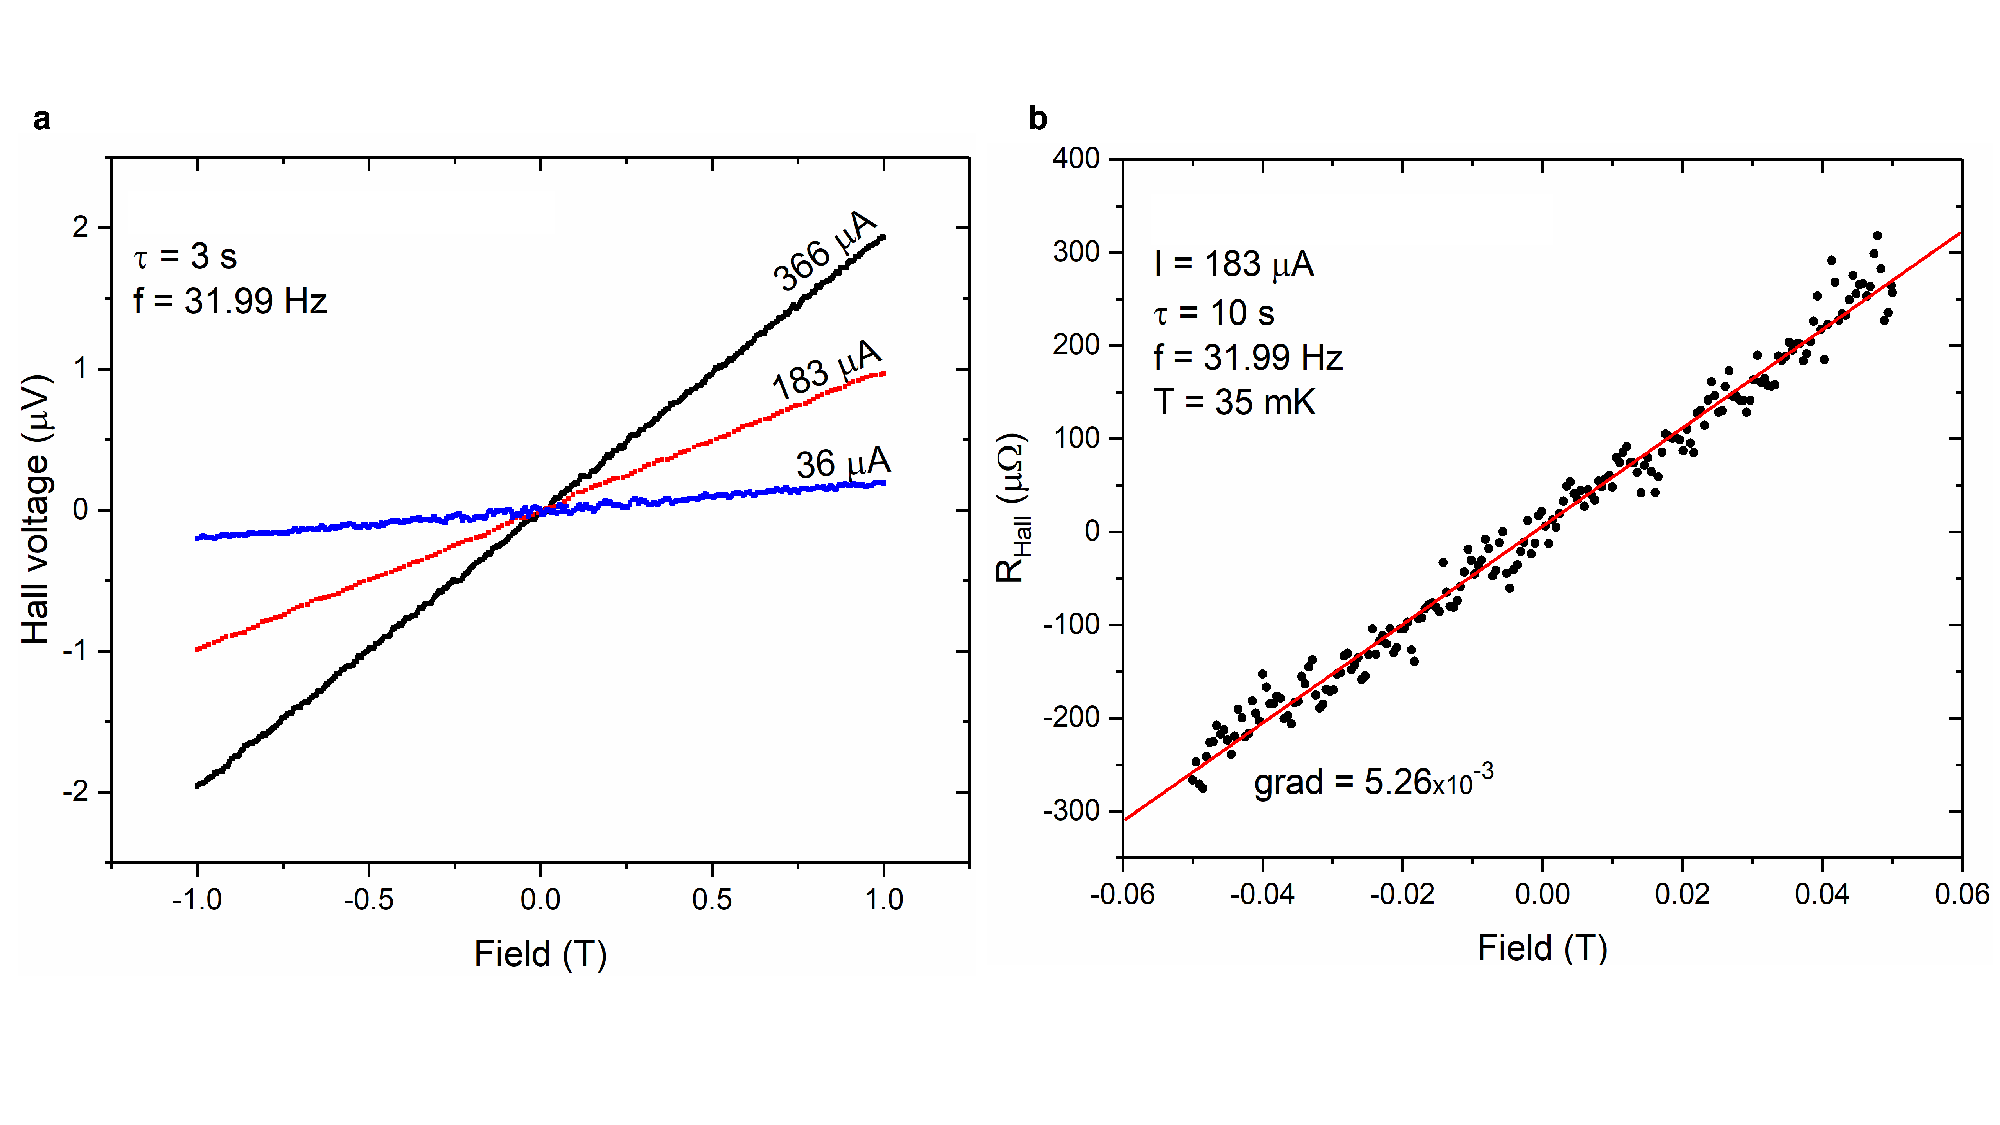
\includegraphics[width=\textwidth]{chapter_fabrication/figures/hall_bar_current_test2.pdf}
        \caption[Driving-Current-Dependent Hall-Voltage Measurements]{\textbf{a,} Hall voltage measured across one cross when the current driven is increased. The signal is proportional to the current as expected. The parameters $f$ and $\tau$ are the lock-in operation frequency and integration time, respectively. The frequency in particular was optimised by taking a frequency scan the line response and set it to the point of minimum noise. \textbf{b,} The Hall coefficient for this particular device was calcualted to be $R_\textrm{H}\sim \SI{1e-6}{\ohm}$G$^{-1}$ which is expected for an Au probe of $d \sim \SI{1}{\micro\metre}$}
        \label{fig:exp:hallbar_test_current}
    \end{center}
\end{figure}

% comment: to calculate the Hall coeff I did the following
% first I looked at the number it was generated from the formula from candini's thesis
% i then used that value and plug it into a converter to estimate the correspondent Gauss
% saw the result was around 6e-6 which is a factor off about the 1e-7 ohm/G reported in this thesis.
% so I plugged in my probe thickness and did the same taking into account that one factor off and 
%found the final result.

\subsubsection{Anisotropy Test}

\begin{figure}[hbtp]
    \begin{center}
        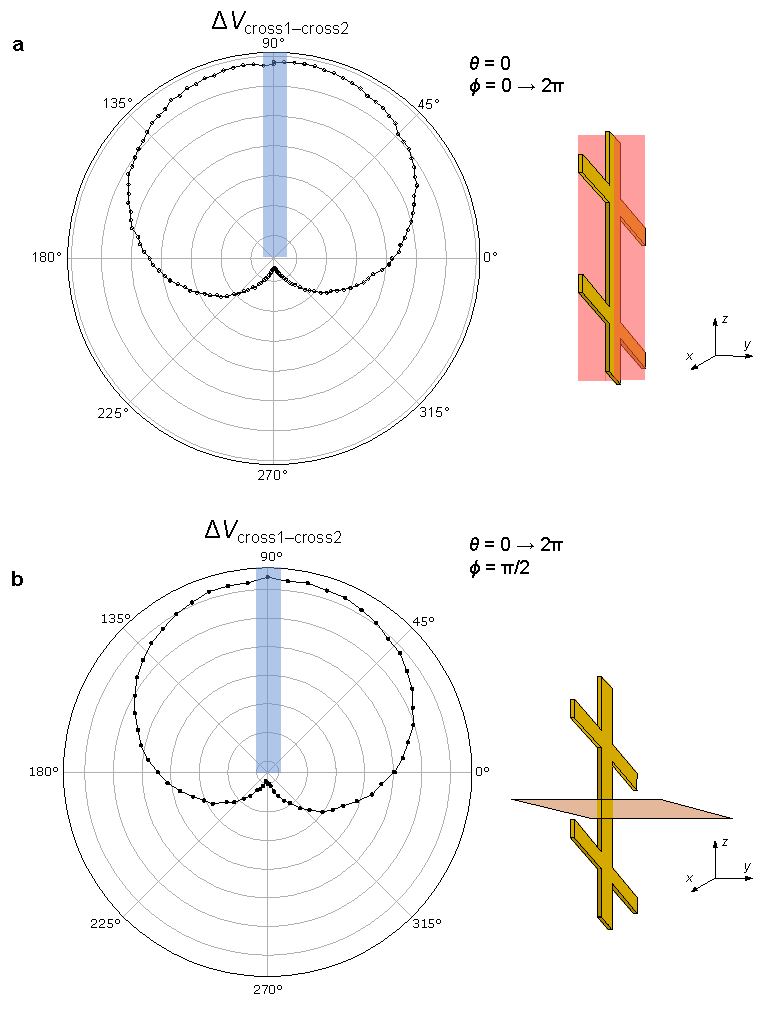
\includegraphics[width=\textwidth]{chapter_fabrication/figures/anisotropy_device.pdf}
        \caption[Angular Relation to Hall Voltage Response]{\textbf{a,} The difference between the voltages build up across the two crosses was recoded thorugh angle-resolved experiments. The direction of maximum signal is highlighted by the blue rectangle and along the $y$ axis, as expected from the Hall effect. On the right, a schematic along which normal-plane the magnet was rotated along. $\theta$ and $\phi$ are the sperhical parameters to input in the routine I wrote. \textbf{b,} polar plot of the response for a $x$-oriented normal-plane. Once again, the region of maximum signal is found when the magnetic field component is perpendicular to the surface of the two crosses.}
        \label{fig:exp:hallbar}
    \end{center}
\end{figure}

\begin{figure}[hbtp]
    \begin{center}
        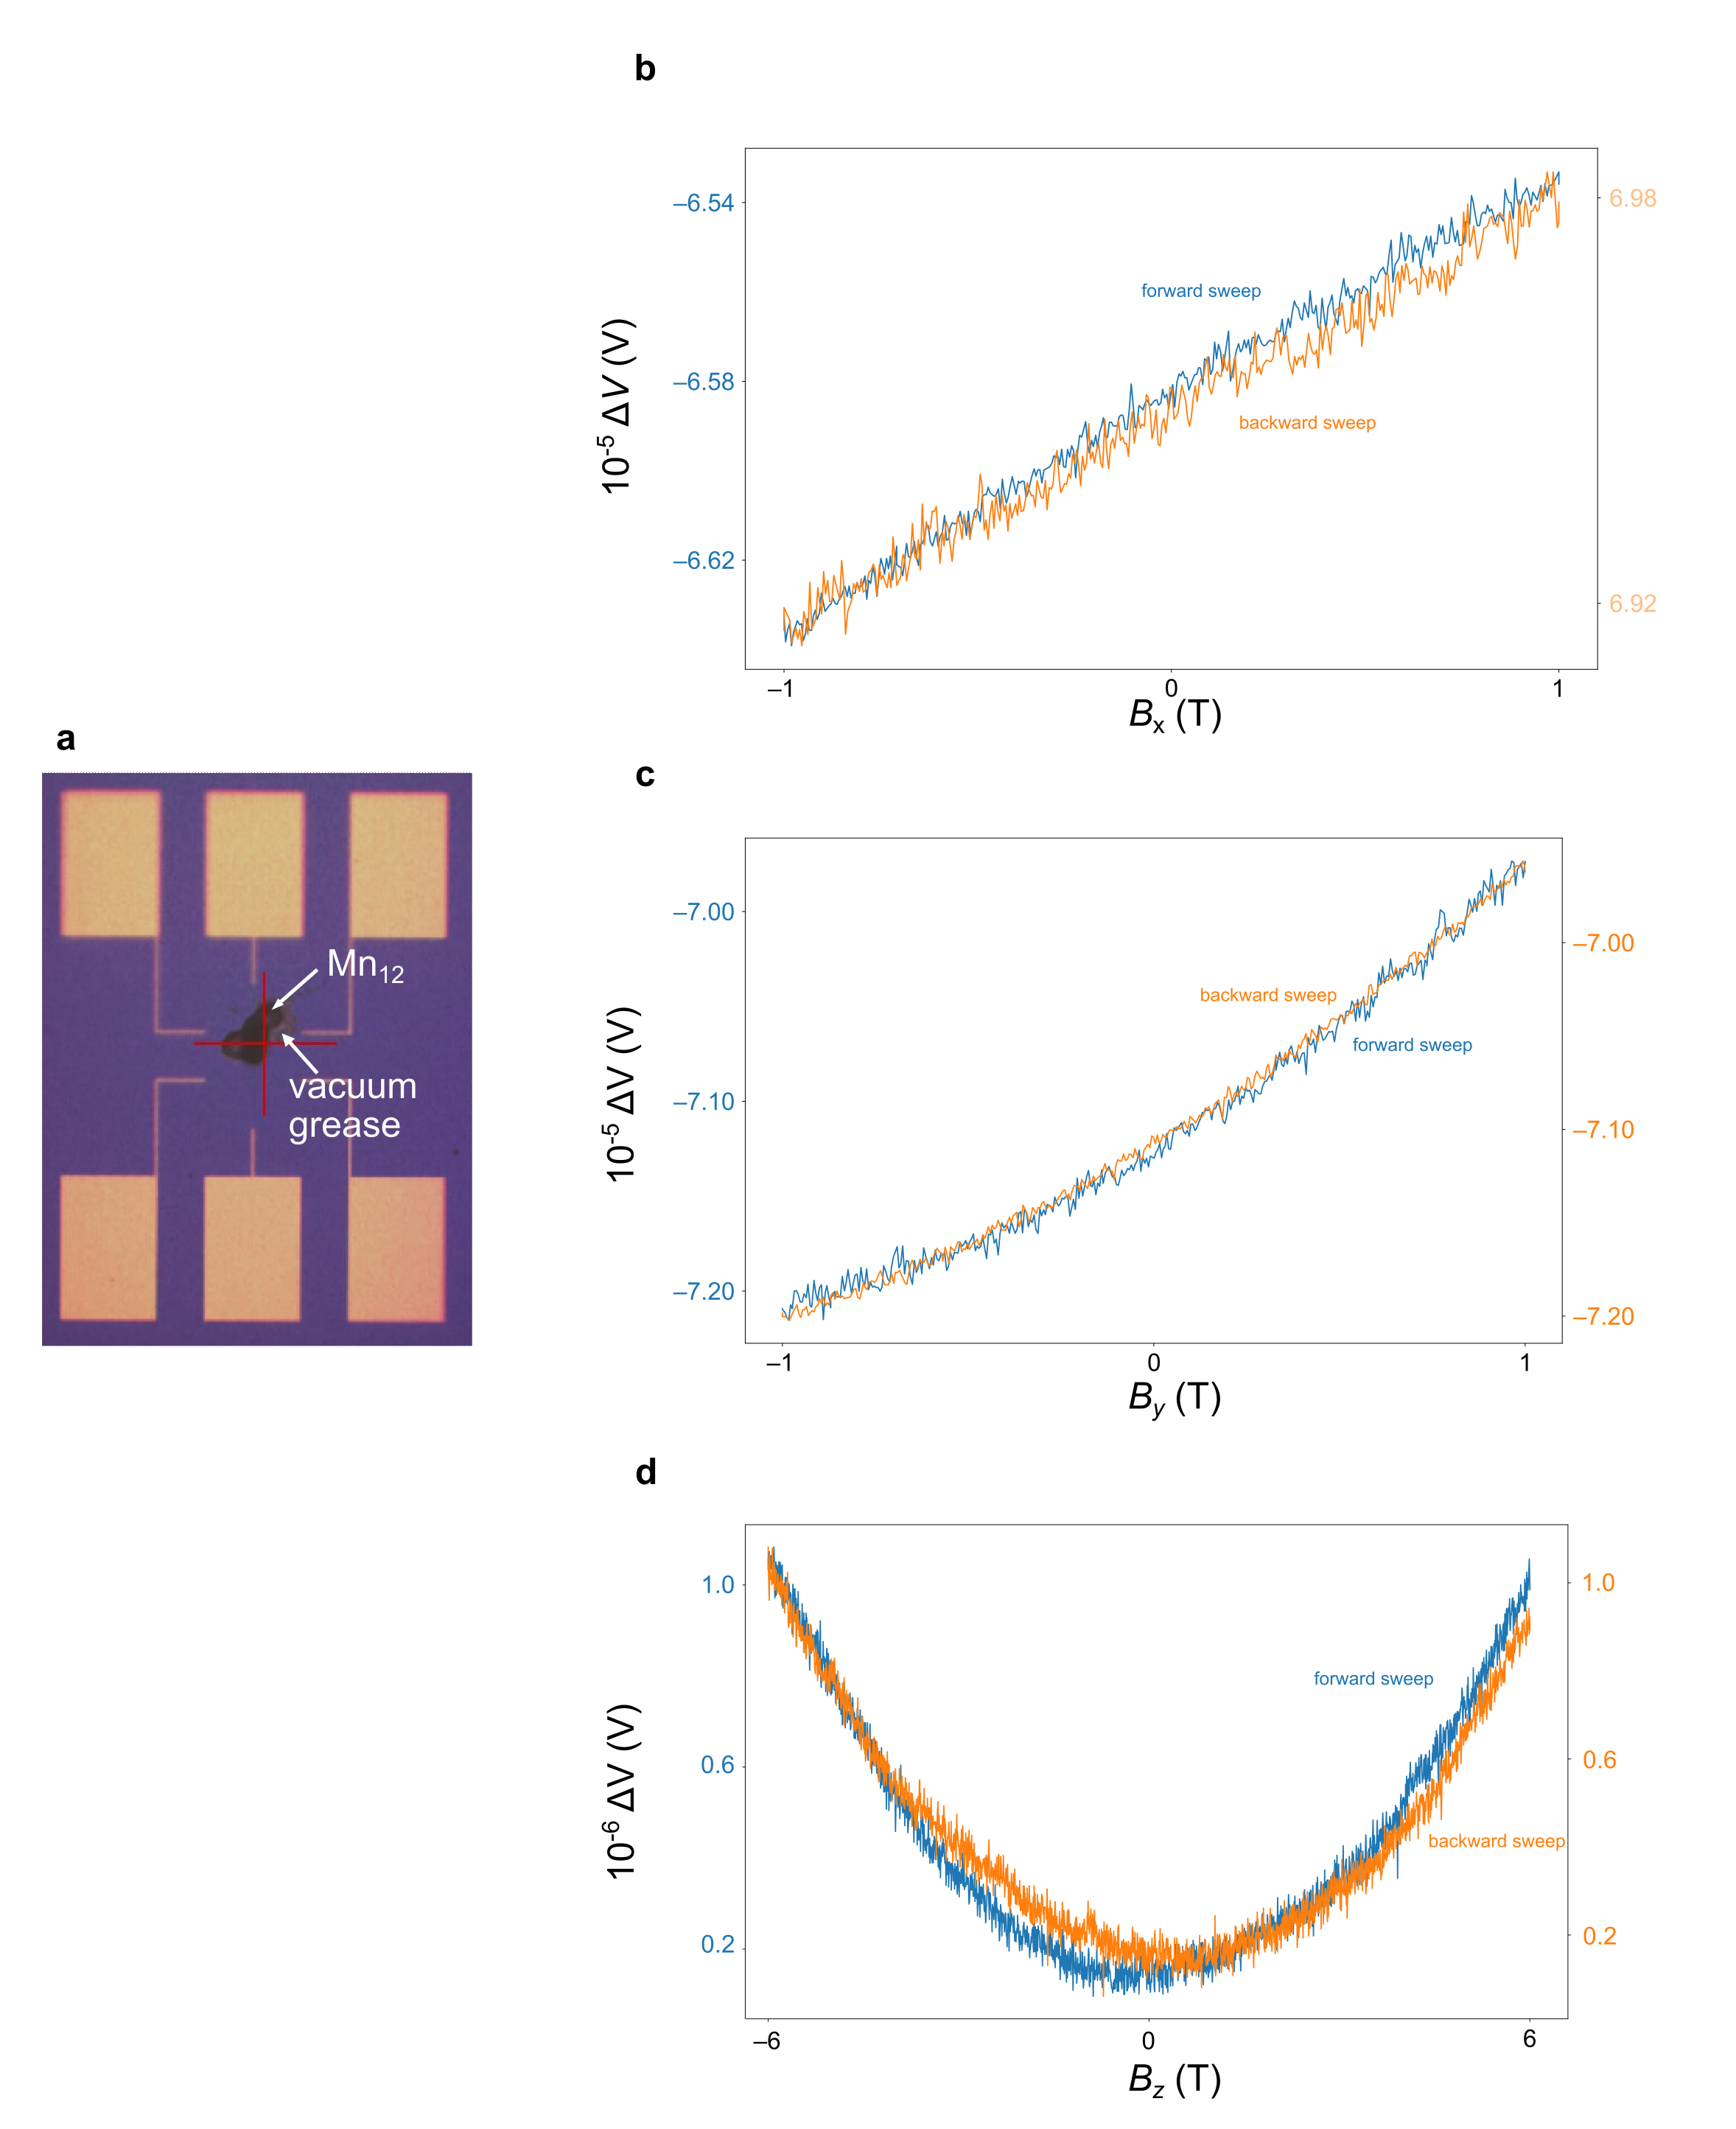
\includegraphics[width=\textwidth]{chapter_fabrication/figures/Mn12_sample2.png}
        \caption[Hall Probe Magnetometry of \ce{Mn12}-ac Micro-Crystals]{
            Cartoon of a micro-Hall sensor. Current flows along the central wires, while the sample sits on one of the two crosses. The sample is placed slightly offset compared to the crossposition as the magnetic field is less shielded by the gold surface. The signals are then measured in parallel by feeding first the voltage drops to two pre-amplifier and later to lock-in amplifiers.}
        \label{fig:exp:hallbar_design}
    \end{center}
\end{figure}

\subsection{Graphene Hall Bars}

To completed

\section{Project Overview}
I thanks Dr\. Alex Gee for his help and expertise substrate fabrication and instrumentation setup.